%% The following is a directive for TeXShop to indicate the main file
%%!TEX root = diss.tex

\chapter{Introduction}
\label{ch:Introduction}

%%%%%
\section{Motivation}

% why are we interested in organic semiconductors
%   various applications, focusing specifically on OPV and OLED

% what is the interesting physics that we want to probe

In the midst of the rapid development of silicon-based and inorganic semiconductors, starting from the early 1900s and have since led to age of modern computing and electronics, the first conducting organic polymer, polyacetylene, was synthesized in 1977 \citep{shirakawa1977synthesis,chiang1977electrical}. The discovery of non-insulating organic plastics established a new research area focused on the development of organic semiconductors, and led to the Chemistry Nobel Prize in 2000 awarded to their discoverers Heeger, MacDiarmid, and Shirakawa. After several decades of research, the class of semiconducting organic molecules have grown substantially, and organic semiconductors have found success in commercial applications such as \acp{OLED} \citep{zhu2011solution,ying2014white}, organic field effect transistors \citep{torsi2013organic,tatum2018pi}, and \acp{OPV} \citep{holliday2017recent,espinosa2015solution,gregg2003comparing,lewis2007toward}. 

The major advantage of organic semiconductors when compared to their inorganic counterparts is their relative ease of processing. Organic molecules can be thermally deposited or solution processed, allowing for cost-effective device fabrication \citep{yip2012recent,huang2019organic}. Additionally, by drawing from a suite of chemical synthesis techniques, new molecules can be created from Earth-abundant organic elements, and engineered with different functional groups to have the desired optical, electronic, and structural properties. This versatility allows for tunable light absorption and emission, transparency, and mechanical flexibility, which have already been applied to niche commercial products (\autoref{fig:intro:applications}). 

\begin{figure}[h]
    \centering
    
    \begin{subfigure}[t]{0.43\textwidth}
        \centering
        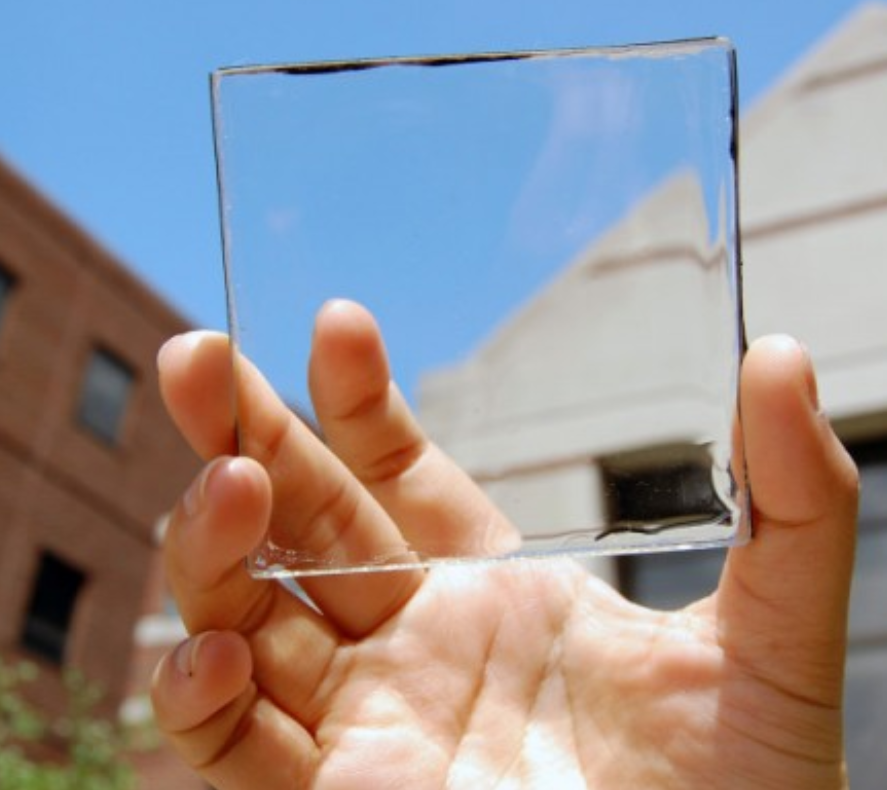
\includegraphics[width=0.8\textwidth]{pictures/transparent_solar.PNG}
        \caption{}
    \end{subfigure}
    \hspace{0.5cm}
    \begin{subfigure}[t]{.43\textwidth}
        \centering
        
\includegraphics[width=\textwidth]{pictures/flexible_opv.jpg}
        \caption{}
    \end{subfigure}
    
    
    \vspace{0.2cm}
    
    \begin{subfigure}[t]{.43\textwidth}
        \centering
        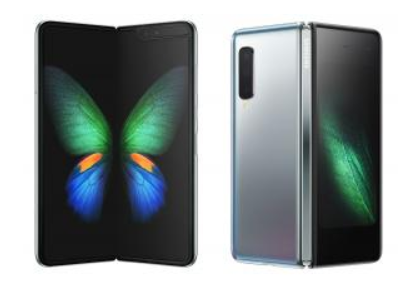
\includegraphics[width=\textwidth]{pictures/folding_oled_fold.PNG}
        \caption{}
    \end{subfigure}
    \hspace{0.5cm}
    \begin{subfigure}[t]{.43\textwidth}
        \centering
        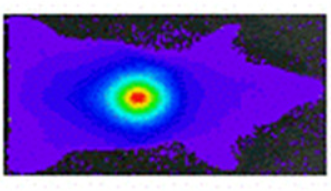
\includegraphics[width=0.95\textwidth]{pictures/biological_oled.PNG}
        \caption{}
    \end{subfigure}
    
    
    \caption[Various applications of organic semiconducting molecules. \textbf{(a)} Organic solar cell that absorbs in the infrared range, making it transparent to visible light. \textbf{(b)} Flexible thin film {OPV} that are fabricated in large rolls (Infinity PV). \textbf{(c)} Foldable display made possible by flexible {OLED} displays (Samsung Electronics). \textbf{(d)} Biological imaging application of {OLED} molecules attached to nanoparticles.]{Various applications of organic semiconducting molecules. \textbf{(a)} Organic solar cell that absorbs in the infrared range, making it transparent to visible light (\citeauthor{zhao2014near} \citep{zhao2014near}). \textbf{(b)} Flexible thin film {OPV} that are fabricated in large rolls (Infinity PV \citep{jacobyInfinityPV}). \textbf{(c)} Foldable display made possible by flexible {OLED} displays (Samsung Electronics \citep{galaxyFold}). \textbf{(d)} Biological imaging application of {OLED} molecules attached to nanoparticles \citep{crossley2017post}.  }
    \label{fig:intro:applications}
\end{figure}

Despite advantages in manufacturing and versatility, organic materials possess low electronic screening, a result of their intrinsically low dielectric constant (or low electric susceptibility), which presents challenges in optimising device performance \citep{gregg2003comparing}. Particularly, in the application of photovoltaics, the photoexcitation of \acp{OPV} results in negatively charged electrons that are bound by the electric force to the positively charge holes left behind. The tightly-bound neutral electron-hole pairs, or \emph{excitons}, make charge extraction difficult in \acp{OPV}, resulting in low \ac{PCE}. As of 2019, the record \ac{PCE} for an \acp{OPV} cell is $17.4\%$ \citep{Meng2018,Cui2019}, while typical efficiencies are at $\sim 10\%$ \citep{NREL2019champion}. Inorganic photovoltaics consistently have \ac{PCE} $> 20\%$ \citep{NREL2019research}, with the most recent record being $47.1\%$ \citep{Geisz2018}.

%On the other hand, light excitation of inorganic photovoltaics generate unbound electrons and holes, which can separate to the cathode and anode respectively.

Understanding the role of excitons is also important to the development of \ac{OLED} devices. Organic semiconductors emit energy in the form of light when excitons recombine---the excited electron ``falls" back into the hole. The colour and intensity of the emitted light is dependent on the energy and recombination rate of excitons formed in the material. The goal in light emitting applications is to maximize exciton recombination, while tuning the optical properties of the exciton. Understanding the underlying physics of exciton formation, dissociation, and recombination will not only optimize device performance, but contribute to the understanding of excited state phenomena in organic molecules.


% Organic semiconductors are a promising class of materials with a multitude of applications to electronics. 

% Organic semiconductor devices are lightweight, flexible, inexpensive, and easily fabricated when compared to conventional semiconductors \citep{lewis2007toward}. 

% However, in the application to photovoltaics, organic semiconductors are much less efficient than traditional photovoltaics made from silicon, due to the low dielectric constant of organic materials \citep{gregg2003comparing}. In order to optimise the power conversion of these devices, the electronic structures of organic photovoltaic molecules need to be understood at the nanoscale, using scanning probe techniques such as \ac{STM}, and \ac{STS} \citep{binnig1982surface}. 


%%%%%
\section{Excitons in organic semiconductors}

When looking at exciton physics in organic semiconductors, there are several energy scales we need to consider (\autoref{fig:intro:exciton}). The band gap is measured as the energy $E_{gap}$ from the \ac{HOMO} to the \ac{LUMO}, which are analogous to the valence and conductance bands inside a solid-state system, respectively. The energy of the \ac{HOMO} can be characterized by the ionization potential $E_I$, the energy required to excite an electron from the occupied orbital into the vacuum level, and \ac{LUMO} by the electron affinity $E_A$, the energy released by the addition of an electron from the vacuum level into the unoccupied orbital.

Due to the low dielectric constant in organic materials, electric fields between charges are stronger due to lower screening. The attractive Coulomb force between the excited electron and the hole favours the formation of an exciton with a lower energy known as the optical gap $E_{opt}$. The exciton binding energy $E_b$ is the difference between the band gap and the optical gap, and is typically on the order of $\sim \SI{1}{eV}$ for organic semiconductors \citep{knupfer2003exciton}. For excitons to dissociate, enough energy needs to be supplied to overcome the binding energy: thermal energy, which is on the order of $k_B T \sim \SI{0.1}{meV}$ ($k_B$ is the Boltzmann constant), is insufficient for thermal dissociation of excitons in organic materials.

\begin{figure}[h]
    \centering
    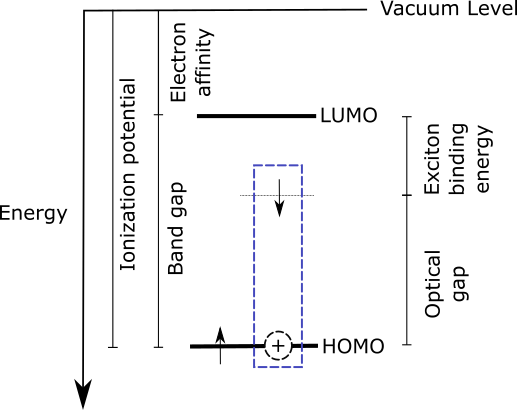
\includegraphics[width=0.7\textwidth]{pictures/exciton_energy.png}
    \caption{Schematic of energy levels involved in photoexcitation in organic semiconducting molecules. The ionization potential, electron affinity, and band gap of the molecule are labelled in the diagram. The optical gap, and exciton binding energy for a photoexcited electron are indicated for a typical exciton.}
    \label{fig:intro:exciton}
\end{figure}

Typically, \ac{OPV} systems are composed of two species of organic semiconducting materials: an electron donor and an electron acceptor molecule. In 1986, \textit{C.W. Tang} demonstrated the importance of the acceptor-donor heterojunction between organic semiconductors to the dissociation of excitons into free charge carriers \citep{tang1986two}. In \acp{OPV}, electrons inside of an organic semiconductor are excited from \ac{HOMO} to the \ac{LUMO} by photons that have energies greater than the band gap of the molecule. Excitons generated in the system act as quasi-particles, and can diffuse as a pair through the material. At the interface, mismatched electron energy levels between the acceptor and donor generate a high electric field that pulls apart the electron-hole pair, similar to the process at p-n junctions in inorganic PV systems. Acceptor organic molecules have high electron affinity, making it energetically favourable for the excited electron to transfer into the acceptor molecule \ac{LUMO} (\autoref{fig:intro:ct}). This delocalizes the exciton between two molecules, forming a \ac{CT} complex, and allows for exciton dissociation and electric current generation in the system \citep{bernardo2014delocalization}.

\begin{figure}[h]
    \centering
    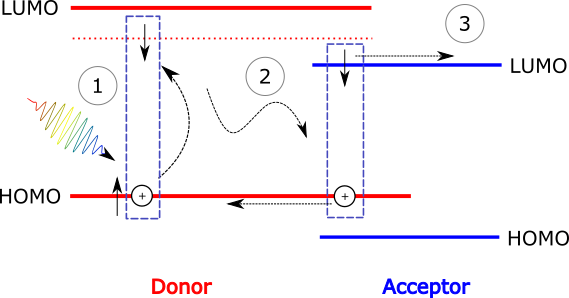
\includegraphics[width=0.8\textwidth]{pictures/CT_energy.png}
    \caption{Schemtic demonstrating the formation of the charge transfer state. \textbf{(1)} An incoming photon excites an electron in the donor system. The exciton forms due to Coulomb force between the electron and hole. \textbf{(2)} Before recombination occurs, the exciton diffuses to the heterojunction. The charge transfer exciton form. \textbf{(3)} With the exciton delocalized, dissociation occurs and the charge is transferred to the acceptor.}
    \label{fig:intro:ct}
\end{figure}

Excitons in \ac{OPV} materials typically have diffusion lengths of 1\SI{-30}{nm} \citep{proctor2013charge}, and have lifetimes ranging from attoseconds to microseconds \citep{tamai2015exciton}. There is a probability of exciton recombination, in which the excited electron drops in energy and re-emits the $E_{opt}$ as light, if the exciton is unable to diffuse to an interface to form the \ac{CT} state. Even after formation of the \ac{CT} complex, recombination can still occur albeit with a different spectroscopic signature.

In light emission applications, the reverse of the photoexcitation process in \acp{OPV} is observed. A year after the two-layer \ac{OPV} publication, \emph{C.W. Tang and S.A. Van Slyke} created the first practical \ac{OLED} device \citep{Tang1987}. Using electron and hole transport layers, charges are directed from the cathode and anode into an emissive layer composed of organic semiconducting molecules, allowing for exciton formation and subsequent recombination. However, complications arise due to the nature of excitons in organic molecules. Vibration modes within the molecule create discrete energy states for each molecular orbital, as described by the Franck-Condon principle (\autoref{fig:intro:vib}). Relaxation between these discrete states can change the energy of the exciton, thereby changing the colour of emitted light.\footnote{This phenomena is described by Kascha's rule. Differences in the absorption and emission spectra can arise, knwon as the Stoke's shift.} Additionally, excited triplet states can form in organic semiconductors, which generally have longer lifetimes and can decay non-radiatively, reducing the efficiency of \ac{OLED} devices. Exciton recombination from triplet states, or phosphorescence, are more rare and lower in energy when compared to recombination from excited singlet states, or fluorescence \citep{kohler2009triplet}.

\begin{figure}[t]
    \centering
    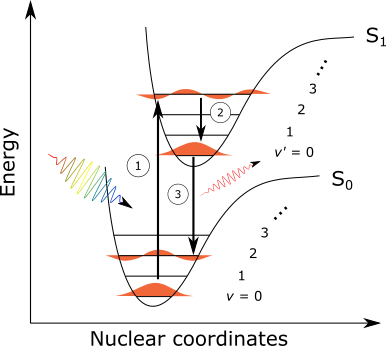
\includegraphics[width=0.7\textwidth]{pictures/franck_condon_transitions.png}
    \caption{Franck-Condon diagram. Vibrational modes are discrete quantum harmonic oscillator levels. \textbf{(1)} Photon excites an electron from singlet ground state into the third mode of the singlet first excited state, the $S_0(\nu=0) \rightarrow S_1(\nu'=3)$ absorption transition. \textbf{(2)} Relaxation in the excited molecule into the lowest vibrational mode $S_1(0)$, reducing the optical gap. \textbf{(3)} Exciton recombination into $S_0(2)$ due to the wavefunction overlap. This diagram demonstrates the $S_1(0) \rightarrow S_0(2)$ fluorescence transition.}
    \label{fig:intro:vib}
\end{figure}



%%%%%
\section{Scanning probe techniques}

% talk about what has been done, and why we should use spm
% Extensive research has been carried out on the optoelectronic properties of organic semiconductors, but often in the context of a device or a bulk ensemble of molecules. However, exciton formation, dissociation, and charge transfer happens on the molecular scale. 

\Acf{SPM} is a suite of experimental characterization techniques that involve measuring the interaction, as a function of experiment parameters, between an extremely sharp probe and some sample. The probe can then be raster scanned, using precise piezoelectric motors, across the sample to give a local spatial map of the interaction, or other determinable quantities. Unlike conventional optical microscopy techniques, \ac{SPM} resolution is determined by the sharpness of the probe which can be as small as a few picometres, allowing for real-space atomically resolved imaging that would not be possible with diffraction limited systems.

Three \ac{SPM} techniques are employed in the work presented in this thesis: \ac{STM}, \ac{STS}, and \ac{STML}, which are all based on the tunnelling of electrons between the a metallic tip and sample, an organic semiconducting molecule supported by a conducting substrate. These three techniques can map out, with atomic resolution, the local structural, electronic, and optical properties of small assemblies of organic semiconducting molecules. The details of the techniques will be discussed in \autoref{ch:exptech}.

Extensive research on organic semiconducting molecules have been conducted, but often in the context of a device, or as a bulk ensemble of molecules. However, changes in heterojunction geometry, local electronic environment, molecular structure, can drastically affect the optoelectronic properties which occur at the nanometre length scale. \ac{SPM} can directly probe these effects at sub-molecular resolution, allowing for correlation between electron and exciton physics with changes in molecular configuration.

%\section{Small molecules }

% In \ac{STM}, atomic resolution topography of the electronic landscape is obtained by measuring fluctations in the tunnelling current as the tip moves across our organic molecule. By sweeping the bias between the tip and the sample, we can identify resonances in the \ac{LDOS} spectroscopy as a function of energy corresponding to molecular orbitals. Performing this \ac{STS} measurement pixel-by-pixel, we can map out the spatial distribution of the occupied and unoccupied molecular states. Additionally, the tunnelling of charges between the tip and sample can generate local excitons in the organic semiconductor. In the \ac{STML} technique, these excitons can be optically detected when they recombine and emit an photon. This permits the mapping of the exciton formation, and, by spectroscopically resolving the emitted photons, the optical gap within the molecule. 

% talk about the disadvantages.
% There are disadvantages to using \ac{SPM} techniques. In particular, \ac{SPM} is highly dependent on the probe; the material and geometry of the probe can affect the measured interaction. The tip can be modified by indentation into a metallic surface, 

% This can affect the quality of topography, spectroscopy, and luminescence signal. Scanning tunnelling techniques also require that the molecules are deposited on a conducting substrate. Molecule-substrate interactions can obscure optoelectronic properties of the free molecule. 

% Additionally, molecule-substrate interaction can affect the 

% As it is difficult to characterize the tip \textit{in situ}, structural and electronic properties of the probe are often approximated with simple models.

% While \ac{SPM} offers high resolution local maps of the sample, the techniques are limited to imaging small select parts of the sample (on the order of $\sim$100 nm). Additionally, the scans are generally slower than other microscopy techniques, meaning that \ac{SPM} techniques generally do not have time resolution, and are susceptible to sample drift, mechanical vibration, and other sources of measurement uncertainty.


% talk about how they are used
% studies that have used SPM for organic molecules before













